\documentclass[11pt]{article}

\usepackage[review]{acl}
\usepackage{times}
\usepackage{latexsym}
\usepackage[T1]{fontenc}
\usepackage[utf8]{inputenc}
\usepackage{microtype}
\usepackage{inconsolata}
\usepackage{graphicx}
\usepackage{booktabs}
\usepackage{tabularx}
\usepackage{array}
\usepackage{multirow}
\usepackage{makecell}
\usepackage{pifont}
\usepackage[table]{xcolor}
\usepackage{amsmath,amssymb}
\usepackage{enumitem}
\usepackage{tcolorbox}
\tcbuselibrary{skins,breakable}
\usepackage{adjustbox}
\usepackage{url}
\usepackage{tikz}
\usetikzlibrary{positioning,arrows.meta,fit,shapes.geometric,calc,decorations.pathreplacing}

\newcommand{\suite}{\textsc{TraceBench}}
\newcommand{\tb}{\textsc{TraceBench-Full}}
\newcommand{\tbh}{\textsc{TraceBench-Hard}}
\newcommand{\cmark}{\ding{51}}
\newcommand{\xmark}{\ding{55}}
\newcommand{\pmark}{$\triangle$}
% Mock-data marker: numbers shown in this color are placeholder previews from
% synthetic data; the final compile after the 4-day server run replaces them
% with real evaluation outputs.
\newcommand{\mockval}[1]{\textcolor{red!75!black}{\textit{#1}}}
\newcolumntype{Y}{>{\centering\arraybackslash}X}
\newcolumntype{L}{>{\raggedright\arraybackslash}X}
\definecolor{TraceBlue}{RGB}{230,240,255}
\definecolor{TraceGreen}{RGB}{232,247,236}
\definecolor{TracePurple}{RGB}{242,238,255}
\definecolor{LightGray}{gray}{0.94}
% Table-cell colors (AlphaDiana-style)
\definecolor{PassGood}{RGB}{220,250,225}      % light green: high Pass@1
\definecolor{PassMed}{RGB}{246,253,235}       % pale green-yellow
\definecolor{BlameLow}{RGB}{253,232,232}      % pale pink: low Blame@1 (bad)
\definecolor{BlameHigh}{RGB}{240,253,244}     % pale green: high Blame@1 (good)
\definecolor{GapLarge}{RGB}{251,212,212}      % pinker: large gap (paper's main claim)
\definecolor{GapMed}{RGB}{254,243,199}        % pale amber: medium gap
\definecolor{OutsideHigh}{RGB}{253,222,222}   % pink: high Outside-G (more diffusion)
\definecolor{OutsideLow}{RGB}{230,245,235}    % light green: low Outside-G
\definecolor{ModelHeader}{RGB}{238,242,255}   % cool blue header for family groups

\newtcolorbox{findingbox}[1]{
  enhanced,
  breakable,
  colback=TracePurple,
  colframe=black!45,
  boxrule=0.6pt,
  arc=1.2mm,
  left=1.4mm,right=1.4mm,top=1.0mm,bottom=1.0mm,
  fonttitle=\bfseries,
  title={#1}
}

\title{TraceBench-Full: Causally Grounded Evaluation of Traceable Multi-Turn Code Debugging}
\author{Anonymous Authors}

% --- All paper-claim numbers flow through numbers.tex (auto-generated
%     by code/scripts/05_render_tex.py). Hand-typed numerics in main.tex
%     are caught by code/scripts/06_consistency_check.py.
% =====================================================================
%  numbers.tex — auto-generated by code/scripts/05_render_tex.py
%
%  DO NOT EDIT this file by hand. Edit the upstream JSON:
%    - REAL  → out/analysis/numbers.json  (produced by `make analyze`)
%    - MOCK  → code/mock_results/mock_bundle.json
%  then re-run `make tex`.
%
%  The current values are MOCK placeholders shown in red italics via
%  \mockval{}. They will be overwritten by `make tex` after a real run.
% =====================================================================

% --- dataset constants (locked) ---
\newcommand{\TBNumModels}{6}%
\newcommand{\TBNumFullProblems}{818}%
\newcommand{\TBNumHardProblems}{128}%
\newcommand{\TBNumFullTurns}{2402}%
\newcommand{\TBNumFullTests}{7165}%
\newcommand{\TBNumFullInjections}{1113}%

% --- Outside-G vs RegressionRate validation ---
%  These are the ONLY place the (r, n, p, CI) for the diffusion-validation
%  claim is defined. main.tex must reference these macros, never type the
%  numbers directly.
\newcommand{\OutsideGRegRCorr}{\mockval{0.62}}%
\newcommand{\OutsideGRegN}{\mockval{2614}}%
\newcommand{\OutsideGRegPValue}{\mockval{< 0.001}}%
\newcommand{\OutsideGRegCILo}{\mockval{0.57}}%
\newcommand{\OutsideGRegCIHi}{\mockval{0.66}}%

% --- early mis-localization → drift (Hit vs Miss) ---
\newcommand{\EarlyDriftCumPatchDelta}{\mockval{+14.2}}%       lines
\newcommand{\EarlyDriftCumPatchCILo}{\mockval{+10.8}}%
\newcommand{\EarlyDriftCumPatchCIHi}{\mockval{+17.6}}%
\newcommand{\EarlyDriftOutsideGDelta}{\mockval{+19.6}}%       points
\newcommand{\EarlyDriftOutsideGCILo}{\mockval{+16.1}}%
\newcommand{\EarlyDriftOutsideGCIHi}{\mockval{+23.0}}%
\newcommand{\EarlyDriftBlameOneDelta}{\mockval{-32.4}}%       points
\newcommand{\EarlyDriftBlameOneCILo}{\mockval{-36.0}}%
\newcommand{\EarlyDriftBlameOneCIHi}{\mockval{-28.7}}%

% --- cost / wall-clock summary ---
\newcommand{\TBGeminiUSDFull}{\mockval{97.4}}%
\newcommand{\TBHonHoursTotal}{\mockval{11.7}}%
\newcommand{\TBCallsTotal}{\mockval{14{,}412}}%

% --- example single-row Gemini stats used in the intro figure caption ---
\newcommand{\GeminiPassFull}{\mockval{91.3}}%
\newcommand{\GeminiBlameFull}{\mockval{39.8}}%
\newcommand{\GeminiGapFull}{\mockval{51.5}}%


\begin{document}
\maketitle

\begin{abstract}
Code agents increasingly solve programming tasks through multi-turn edit-test-revise loops. In this setting, final test success is an incomplete evaluation object: a passing program may result from a localized causal repair, or from a broad trajectory that rewrites verified code, obscures the active fault, and introduces regressions before converging. We study this mismatch as the \emph{traceability gap} in multi-turn code debugging.

We introduce \tb{}, a causally grounded dataset and evaluation suite for traceable debugging. Each instance starts from a verified reference program and is converted into a debugging task through typed semantic fault injection, executable causal checks, active fault spans, counterfactual repair patches, and full transcript logging. The release contains 818 problems, 2402 multi-turn traces, and 7165 test cases; \tbh{} is a 128-instance strict subset for high-signal diagnosis of strong coding agents.

\suite{} evaluates attribution, propagation, and accumulation. Across representative code LLMs, high Pass@1 frequently coexists with weak fault attribution. The gap persists on \tb{} and becomes sharper on \tbh{}. We further validate edit diffusion against newly introduced regressions, showing that process metrics capture harmful trajectory behavior rather than only patch size. We release the data, manifests, evaluation scripts, and documentation for process-level evaluation of code agents.
\end{abstract}

\section{Introduction}
\label{sec:intro}

Modern coding agents solve programming tasks as interactive repair processes. They inspect failures, edit code, rerun tests, and revise under feedback. This changes the evaluation target. A final passing program may be produced by a localized causal repair, or by a broad trajectory that touches verified code, hides the true fault, and leaves the patch difficult to review. Outcome-only metrics treat these trajectories identically.

This blind spot is becoming more important as code agents move from one-shot synthesis to repository and environment interaction. Benchmarks such as SWE-bench and recent long-horizon variants emphasize realistic issue resolution, while new training recipes use pull requests or agent-native rollouts to internalize software-engineering skills into model weights \citep{jimenez2024swebench,deng2025swebenchpro,zhu2026cleanpr,zeng2026davincidev}. These developments raise the capability bar, but they do not answer a process question: \emph{when an agent succeeds, did it repair the right thing in the right place?}

We call this missing information the \emph{traceability gap}. Final correctness does not specify which region the model suspected, whether the edit was causally tied to the active fault, or whether previous progress was preserved across turns. Real issue-resolution benchmarks are realistic but often lack causal fault spans because human patches can mix bug fixes, refactors, and incidental changes. Seeded-bug datasets provide cleaner references but usually lack multi-turn transcripts. Trajectory-aware benchmarks log agent behavior but generally do not make the active fault counterfactually auditable at each failed turn.

We introduce \tb{}, a causally grounded dataset and evaluation suite for traceable multi-turn code debugging. Each instance begins from a verified reference program $P^\star$. We inject typed semantic faults, enforce executable causal checks, and store active fault spans together with minimal counterfactual repair patches. The benchmark logs complete interaction transcripts, blamed spans, turn-level diffs, and test transitions. This makes it possible to evaluate not only whether the final program passes, but also how the repair path localizes, edits, and stabilizes.

\begin{figure*}[t]
\centering
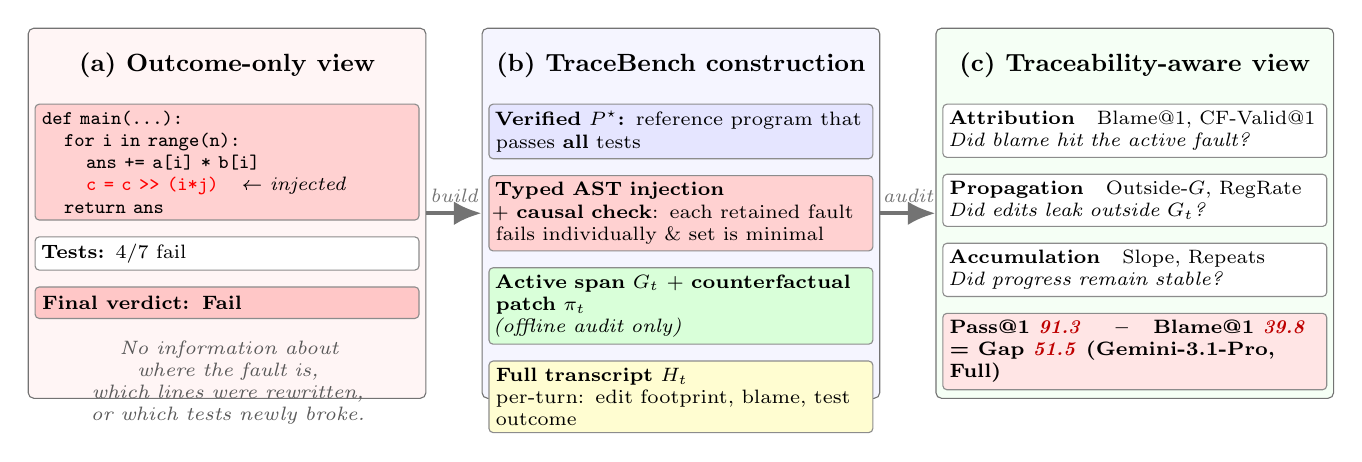
\begin{tikzpicture}[
  font=\footnotesize,
  node distance=4mm and 7mm,
  panel/.style={draw=black!55, rounded corners=2pt, line width=0.4pt,
                inner sep=4pt, minimum width=5.05cm, minimum height=4.7cm,
                fill=#1, align=left},
  paneltitle/.style={font=\bfseries\small},
  box/.style={draw=black!45, rounded corners=1.5pt, fill=white,
              inner sep=2.5pt, align=left, font=\scriptsize, minimum height=4mm},
  hot/.style={fill=red!18},
  ok/.style={fill=green!15},
  cool/.style={fill=blue!10},
  flowarr/.style={-{Latex[length=2.2mm,width=2mm]}, line width=0.6pt, draw=black!70},
  bigarr/.style={-{Latex[length=3.5mm,width=3mm]}, line width=1.4pt, draw=black!55},
]
%====================== PANEL A ======================
\node[panel=red!4] (A) at (0,0) {};
\node[paneltitle, anchor=north] (At) at ([yshift=-2mm]A.north) {(a) Outcome-only view};
\node[box, hot, below=2mm of At, text width=4.7cm] (Acode) {%
\texttt{def main(...):}\\
\quad \texttt{for i in range(n):}\\
\quad\quad\texttt{ans += a[i] * b[i]}\\
\quad\quad\textcolor{red}{\texttt{c = c >> (i*j)}}\quad\textit{← injected}\\
\quad \texttt{return ans}};
\node[box, below=2mm of Acode, text width=4.7cm] (Atest) {\textbf{Tests:} 4/7 fail};
\node[box, below=2mm of Atest, fill=red!22, text width=4.7cm, font=\scriptsize\bfseries] (Averd) {Final verdict: \textsc{Fail}};
\node[below=1.5mm of Averd, text width=4.7cm, align=center, font=\scriptsize\itshape, text=black!65]
     {\,No information about \textit{where} the fault is,\\ \textit{which lines} were rewritten,\\ or \textit{which tests} newly broke.};

%====================== PANEL B ======================
\node[panel=blue!4, right=of A] (B) {};
\node[paneltitle, anchor=north] (Bt) at ([yshift=-2mm]B.north) {(b) \textsc{TraceBench} construction};
\node[box, cool, below=2mm of Bt, text width=4.7cm] (Bref) {\textbf{Verified $P^\star$:} reference program that passes \textbf{all} tests};
\node[box, hot, below=2mm of Bref, text width=4.7cm] (Binj) {\textbf{Typed AST injection}\\ + \textbf{causal check}: each retained fault fails individually \& set is minimal};
\node[box, ok, below=2mm of Binj, text width=4.7cm] (Bcf)  {\textbf{Active span $G_t$} + \textbf{counterfactual patch $\pi_t$}\\ \textit{(offline audit only)}};
\node[box, fill=yellow!18, below=2mm of Bcf, text width=4.7cm] (Btrans) {\textbf{Full transcript $H_t$}\\ per-turn: edit footprint, blame, test outcome};

%====================== PANEL C ======================
\node[panel=green!4, right=of B] (C) {};
\node[paneltitle, anchor=north] (Ct) at ([yshift=-2mm]C.north) {(c) Traceability-aware view};
\node[box, below=2mm of Ct, text width=4.7cm] (Catt) {\textbf{Attribution}\quad Blame@1, CF-Valid@1\\ \textit{Did blame hit the active fault?}};
\node[box, below=2mm of Catt, text width=4.7cm] (Cprop) {\textbf{Propagation}\quad Outside-$G$, RegRate\\ \textit{Did edits leak outside $G_t$?}};
\node[box, below=2mm of Cprop, text width=4.7cm] (Cacc) {\textbf{Accumulation}\quad Slope, Repeats\\ \textit{Did progress remain stable?}};
\node[box, fill=red!10, below=2mm of Cacc, text width=4.7cm, font=\scriptsize\bfseries] (Cgap) {Pass@1 \mockval{91.3} \quad\textendash\quad Blame@1 \mockval{39.8} \\ = \textbf{Gap \mockval{51.5}} (Gemini-3.1-Pro, Full)};

%====================== ARROWS BETWEEN PANELS ======================
\draw[bigarr] (A.east) -- node[above, font=\scriptsize\itshape, text=black!55] {build}    (B.west);
\draw[bigarr] (B.east) -- node[above, font=\scriptsize\itshape, text=black!55] {audit}    (C.west);
\end{tikzpicture}
\caption{\textbf{From outcome-only to traceability-aware debugging evaluation.}
(a) A passing trajectory under outcome-only evaluation collapses into one Pass/Fail bit.
(b) \suite{} starts from a verified reference $P^\star$, injects typed semantic faults under individual-failure and setwise-minimality checks, and stores active fault spans $G_t$ plus minimal counterfactual repair patches $\pi_t$ together with the full transcript $H_t$.
(c) These offline labels make a per-turn audit possible along three axes (attribution / propagation / accumulation). Even a strong frontier agent often passes the final test while leaving a substantial Pass$-$Blame gap.}
\label{fig:overview}
\end{figure*}

The release separates \emph{coverage} from \emph{diagnosis}. \tb{} contains 818 problems, 2402 traces, and 7165 test cases, spanning easy through extreme tasks. \tbh{} is a strict 128-instance subset selected after the same causal validity checks to stress-test strong agents on hard, very-hard, and extreme cases. The full split asks whether the traceability gap persists at scale. The hard split asks how strong models behave when raw coding ability is not the only bottleneck.

\paragraph{Contributions.}
\begin{itemize}[leftmargin=*,nosep]
    \item We introduce \tb{}, a causally grounded data resource for traceable multi-turn code debugging, with a broad full split and a high-signal hard split.
    \item We provide a verify-inject-check-log construction pipeline that records active fault spans, counterfactual repairs, fault families, full transcripts, and turn-level edit footprints.
    \item We define a compact evaluation protocol for attribution, propagation, and accumulation, including behavioral validation that structural edit diffusion correlates with newly introduced regressions.
    \item We benchmark representative code LLMs and show that final success and traceable repair diverge: the gap persists on \tb{} and is amplified on \tbh{}.
\end{itemize}

\section{Why Existing Benchmarks Are Not Enough}
\label{sec:positioning}

\begin{table*}[t]
\centering
\small
\setlength{\tabcolsep}{3.1pt}
\renewcommand{\arraystretch}{1.10}
\caption{\textbf{Benchmark matrix motivating \suite{}.} Existing resources cover important pieces of code-agent evaluation, but none jointly provides multi-turn executable traces, controlled causal faults, active fault spans, counterfactual repair labels, and turn-level diffusion metrics. \cmark{} = available, \pmark{} = partial/proxy, \xmark{} = not provided.}
\label{tab:benchmark-matrix}
\begin{adjustbox}{max width=\textwidth}
\begin{tabular}{@{}p{3.05cm}p{3.45cm}ccccccp{4.3cm}@{}}
\toprule
\textbf{Resource} & \textbf{Primary target} & \makecell{Multi-\\turn} & \makecell{Exec.\\feedback} & \makecell{Controlled\\fault} & \makecell{Active\\fault span} & \makecell{Counterf.\\repair} & \makecell{Turn-level\\diffusion} & \textbf{Remaining gap for traceable debugging} \\
\midrule
HumanEval / MBPP / APPS / CodeContests \citep{chen2021humaneval,austin2021program,hendrycks2021apps,li2022alphacode} & One-shot functional synthesis & \xmark & \pmark & \xmark & \xmark & \xmark & \xmark & Measures whether code passes tests, not how a repair trajectory localizes or preserves correct regions. \\
LiveCodeBench / EvalPlus \citep{jain2024livecodebench,liu2023evalplus} & Stronger functional testing and contamination-aware evaluation & \pmark & \cmark & \xmark & \xmark & \xmark & \xmark & Strengthens final correctness but still lacks causal repair-state supervision. \\
\midrule
Defects4J / BugsInPy \citep{just2014defects4j,widyasari2020bugsinpy} & Real or historical program repair & \xmark & \cmark & \xmark & \pmark & \pmark & \xmark & Human fixes provide patch lines, but active causal fault spans and multi-turn drift are not logged. \\
SWE-bench / Verified \citep{jimenez2024swebench,openai2024swebenchverified} & Repository issue resolution & \pmark & \cmark & \xmark & \pmark & \pmark & \pmark & Realistic patches can mix root fixes, refactors, and incidental changes. \\
SWE-Bench Pro \citep{deng2025swebenchpro} & Long-horizon enterprise-level issue resolution & \cmark & \cmark & \xmark & \pmark & \pmark & \pmark & Excellent capability stress test, but natural patches do not expose counterfactual active-fault labels. \\
\midrule
QuixBugs / DebugBench \citep{lin2017quixbugs,tian2024debugbench} & Seeded or paired debugging tasks & \xmark & \cmark & \cmark & \cmark & \pmark & \xmark & Controlled faults exist, but trajectories, history, and edit diffusion over turns are absent. \\
InterCode / CodeFlowBench \citep{yang2023intercode,wang2025codeflowbench} & Interactive code construction with execution feedback & \cmark & \cmark & \xmark & \xmark & \xmark & \pmark & Interaction is visible, but there is no pre-existing active fault with a counterfactual repair target. \\
Terminal-Bench \citep{merrill2026terminalbench} & Realistic command-line agent tasks & \cmark & \cmark & \xmark & \xmark & \xmark & \pmark & Logs commands and outcomes, but not causal repair spans or offline attribution labels. \\
ContextBench / RACE-bench / TRAJEVAL / CodeTracer \citep{li2026contextbench,liu2026racebench,kim2026trajeval,li2026codetracer} & Process-oriented context, reasoning, or trajectory diagnosis & \cmark & \cmark & \xmark & \pmark & \pmark & \pmark & Provides process labels or reference-patch structure, but not controlled active-fault counterfactuals at each failed turn. \\
Clean-PR / daVinci-Dev \citep{zhu2026cleanpr,zeng2026davincidev} & Training data for repo-level or agent-native SWE ability & \pmark & \pmark & \xmark & \xmark & \xmark & \xmark & Helps internalize capability into weights; not an evaluation resource for causal traceability. \\
\rowcolor{TraceBlue}
\suite{} (ours) & Causally grounded traceable multi-turn debugging & \cmark & \cmark & \cmark & \cmark & \cmark & \cmark & Designed to measure attribution, propagation, and accumulation under full transcripts and executable causal checks. \\
\bottomrule
\end{tabular}
\end{adjustbox}
\end{table*}

Table~\ref{tab:benchmark-matrix} is the main positioning claim. Prior resources optimize different axes: outcome-centric benchmarks test functional synthesis, repository benchmarks maximize realism, seeded-bug datasets provide clean fixes, and recent process-oriented benchmarks expose context retrieval or trajectory stages. \suite{} targets the missing intersection: multi-turn executable repair with active fault spans and counterfactual repairs available for offline audit.

\paragraph{Relation to concurrent controller work.}
A concurrent paper studies a CLI repair environment and an inference-time controller for traceable repair \citep{anonymous2026tracebenchcli}. This submission addresses a different contribution: the \tb{} data resource, its full/hard split design, construction validity, metric protocol, and benchmark-wide analysis. Controller-based steering can be evaluated with the released traces, but it is not the main contribution of this paper.

\section{TraceBench-Full}
\label{sec:tracebench}

\suite{} turns process-level debugging evaluation into a controlled data problem. Three challenges guide the construction.
\begin{enumerate}[leftmargin=*,nosep]
    \item \textbf{Ambiguous repair state.} A terminal label does not reveal the active fault, the intended edit scope, or whether regressions accumulated during the run.
    \item \textbf{Fragile trajectory comparison.} Agents may see different histories, budgets, or hints, making process metrics hard to compare unless the protocol is fixed.
    \item \textbf{Causal supervision.} Human patches are realistic but rarely identify which single span is responsible for the current failed turn.
\end{enumerate}
\suite{} addresses these challenges with a verified reference program, typed fault injection, causal checks, and replayable transcripts.

\paragraph{Construction pipeline.}
For each programming task, we obtain a verified reference program $P^\star$ and validate it with executable tests. We parse $P^\star$ into structural units, build fixed unit and end-to-end tests, and inject typed semantic faults through AST-level transformations. Each injection stores the fault family, the clean span, the buggy span, and the minimal counterfactual patch back to $P^\star$. We retain an instance only if each injected fault fails individually and the multi-fault set is setwise minimal: no strict subset of faults explains the retained failures. This conservative filter reduces raw scale but ensures that every retained instance supports causal attribution and counterfactual replay.

\begin{table}[t]
\centering
\small
\setlength{\tabcolsep}{4pt}
\caption{Benchmark splits. \tbh{} is a strict high-signal subset of \tb{}, not the full benchmark size.}
\label{tab:splits}
\begin{adjustbox}{max width=\linewidth}
\begin{tabular}{lrr}
\toprule
\textbf{Statistic} & \textbf{\tb{}} & \textbf{\tbh{}} \\
\midrule
Problems & 818 & 128 \\
Rating mean / median & 1699 / 1600 & 2679.7 / 2700 \\
Depth mean & 3.20 & 3.75 \\
Total turns & 2402 & 442 \\
Avg turns / problem & 2.94 & 3.45 \\
Total subproblems & 2743 & 549 \\
Total test cases & 7165 & 1511 \\
Avg injections / problem & 1.36 & 1.40 \\
Multi-turn coverage & 100\% & 100\% \\
\bottomrule
\end{tabular}
\end{adjustbox}
\end{table}

\paragraph{Evaluation record.}
A \suite{} run stores an auditable record
\[
R=(x,P^\star,P_0,\mathcal{T},\mathcal{G},\Pi,\tau,s),
\]
where $x$ is the problem statement, $P_0$ is the faulty program, $\mathcal{T}$ is the fixed test suite, $\mathcal{G}$ is the set of stored fault spans, $\Pi$ is the set of counterfactual repairs, $\tau$ is the full interaction transcript, and $s$ contains outcome and process scores. The oracle objects $\mathcal{G}$ and $\Pi$ are used only for offline evaluation; they are not exposed to the model.

\section{Protocol and Metrics}
\label{sec:metrics}

\paragraph{Transcript-visible protocol.}
Let
\[
H_t=(P_0,O_0,A_0,P_1,O_1,A_1,\ldots,P_t,O_t)
\]
denote the complete interaction transcript before submission $t$, including prior program states, model submissions, parsed blamed spans, execution feedback, tracebacks, and test outputs. Every method receives the same $H_t$ and produces a revised program $P_{t+1}$ plus optional blamed spans. We use $(P_t,O_t)$ only as metric variables; they are not the full prompt context. Drift in \suite{} is therefore not caused by resetting the prompt, but by failures to use available long-context evidence and prior feedback effectively.

\begin{table}[t]
\centering
\small
\setlength{\tabcolsep}{3pt}
\caption{Primary process metrics. Secondary metrics and edge cases are in Appendix~\ref{app:metrics}.}
\label{tab:metrics}
\begin{tabularx}{\linewidth}{@{}p{1.75cm}p{2.35cm}L@{}}
\toprule
\textbf{Axis} & \textbf{Primary metric} & \textbf{Operational meaning} \\
\midrule
Attribution & Blame@1, CF-Valid@1 & Does the top blamed span overlap the active fault, and does reverting that overlap repair the current failure? \\
Propagation & Outside-$G$, RegressionRate & Do edits diffuse outside the grounded fault neighborhood, and do they break tests that previously passed? \\
Accumulation & Progress slope, $R^2$, repeats & Does the trajectory steadily improve, or does it oscillate through repeated edits, tests, and regressions? \\
\bottomrule
\end{tabularx}
\end{table}

\paragraph{Attribution.}
At each failed turn, \suite{} identifies an active fault span $G_t$: the stored span whose counterfactual revert resolves the currently observed failing assertion while leaving other lines unchanged. The model outputs up to $K$ blamed spans. Blame@1 checks whether the top span overlaps $G_t$. CF-Valid@1 applies the corresponding counterfactual intervention and reruns the relevant test, separating superficial overlap from causal diagnosis.

\paragraph{Propagation and accumulation.}
Let $E_t$ be the line-level edit footprint from $P_t$ to $P_{t+1}$. Outside-$G$ is the fraction of edited lines outside the grounded fault neighborhood. We treat it as a structural diffusion proxy, not a generic penalty on patch size. To validate semantic relevance, we compute RegressionRate: the fraction of tests that passed before the edit but fail after the edit. We also record pass-ratio progress $\rho(P_t)=\#\mathrm{passed}(P_t)/|\mathcal{T}|$, repeated submissions, tests without intervening edits, and trajectory slope/$R^2$. These metrics are reported as components rather than collapsed into a single score.

\section{What TraceBench-Full Reveals}
\label{sec:findings}

\paragraph{Experimental setup.}
The main analysis uses the same staged multi-turn protocol on both splits. At each turn, the model receives the full transcript $H_t$, the current runnable program, the fixed tests, and the latest failure output, then returns a revised program and optional blamed spans. The harness executes the submitted program, records the edit footprint, updates the transcript, and stops on the first full pass. We report Pass@1 for final success, Blame@1 for top-span attribution, Outside-$G$ for diffusion, and RegressionRate for newly introduced failures. Hard-split confidence intervals are task-bootstrap 95\% intervals over fixed single-run trajectories; they quantify instance-level uncertainty rather than decoding-seed variance, which is appropriate for a dataset paper.

\subsection{Outcome-Based Analysis}
\label{sec:outcome-analysis}

\paragraph{Status of numerical results.}
Throughout Section~\ref{sec:findings} and Appendix~\ref{app:full-results}, mock placeholder numbers from a synthetic pre-run are shown in \mockval{red italics}. These will be replaced by real values after the four-day server run described in Appendix~\ref{app:protocol}.

Table~\ref{tab:gap} reports the main outcome-traceability contrast. We evaluate six representative code LLMs on both splits under the same transcript-visible protocol: five open-weight models that run on a single H100 80\,GB GPU (two Qwen dense flagship models, two mixture-of-experts models, one reasoning-distilled model) and one closed-source frontier model accessed via the Gemini API. The six rows are drawn from four model families (Qwen dense, Qwen MoE, GLM MoE, DeepSeek reasoning) plus the closed Gemini vendor, so any persistent Pass--Blame gap cannot be attributed to a single architecture or training recipe. Each model is run once on \tb{}; \tbh{} rows are derived from the same trajectories by filtering the per-problem records by \texttt{problem\_id}, since \tbh{} is a strict subset of \tb{} (128/128 overlap; identical injections and turns for shared problems). Two findings emerge.

\begin{findingbox}{Finding 1. High final success can coexist with weak attribution.}
Adding easier coverage raises Pass@1, but does not eliminate the Pass--Blame gap. The gap persists across all six current models on \tb{} and becomes sharper on \tbh{} for most rows, even though the protocol gives every model the same full transcript $H_t$ and parses blamed spans from the same JSON schema.
\end{findingbox}

\begin{table*}[t]
\centering
\small
\setlength{\tabcolsep}{3.8pt}
\renewcommand{\arraystretch}{1.18}
\caption{\textbf{Main results across six models on \tb{} (818 problems) and \tbh{} (128 high-signal subset).} Attribution: Blame@1, Blame@3, CF-Valid@1. Propagation: Outside-$G$, RegressionRate. Accumulation: average turns to early stop, repeats, per-trajectory progress slope. \tbh{} rows are derived from the same \tb{} trajectories by filtering on \texttt{problem\_id} (verified 128/128 overlap). Hard Gap reports task-bootstrap 95\% CI over fixed single-run trajectories. Cell shading: green = good, pink = bad along each metric's natural direction (note: low Blame = bad; high Out-$G$ = bad). Numbers in \mockval{red italics} are placeholder mocks.}
\label{tab:gap}
\begin{adjustbox}{max width=\textwidth}
\begin{tabular}{l@{\hspace{6pt}}c@{\hspace{6pt}}c@{\hspace{6pt}}|rrr|rr|rrr|r}
\toprule
 & & & \multicolumn{3}{c|}{\textbf{Attribution}} & \multicolumn{2}{c|}{\textbf{Propagation}} & \multicolumn{3}{c|}{\textbf{Accumulation}} & \\
\textbf{Model} & \textbf{Access} & \textbf{Split} & \textbf{Pass@1} & \textbf{Blame@1} & \textbf{Blame@3} & \textbf{Out-$G$} & \textbf{RegR.} & \textbf{AvgT.} & \textbf{Reps.} & \textbf{Slope} & \textbf{Gap} \\
\midrule
\rowcolor{ModelHeader}\multicolumn{12}{l}{\textit{Open dense}}\\
Qwen3.5-27B                  & local & \tb{}  & \cellcolor{PassMed}\mockval{72.4} & \cellcolor{BlameLow}\mockval{38.2} & \mockval{51.7} & \cellcolor{OutsideLow}\mockval{18.3} & \mockval{12.1} & \mockval{2.81} & \mockval{0.42} & \mockval{0.118} & \cellcolor{GapMed}\mockval{34.2} \\
Qwen3.5-27B                  & local & \tbh{} & \cellcolor{PassMed}\mockval{51.6} & \cellcolor{BlameLow}\mockval{17.4} & \mockval{27.3} & \cellcolor{OutsideHigh}\mockval{29.7} & \mockval{18.5} & \mockval{3.40} & \mockval{0.61} & \mockval{0.085} & \cellcolor{GapMed}\mockval{34.2$\pm$6.1} \\
Qwen3.6-27B                  & local & \tb{}  & \cellcolor{PassGood}\mockval{81.5} & \cellcolor{BlameLow}\mockval{42.7} & \mockval{58.4} & \cellcolor{OutsideLow}\mockval{16.9} & \mockval{10.4} & \mockval{2.62} & \mockval{0.35} & \mockval{0.137} & \cellcolor{GapMed}\mockval{38.8} \\
Qwen3.6-27B                  & local & \tbh{} & \cellcolor{PassMed}\mockval{64.8} & \cellcolor{BlameLow}\mockval{21.2} & \mockval{32.6} & \cellcolor{OutsideHigh}\mockval{27.4} & \mockval{16.8} & \mockval{3.29} & \mockval{0.54} & \mockval{0.094} & \cellcolor{GapLarge}\mockval{43.6$\pm$5.3} \\
\midrule
\rowcolor{ModelHeader}\multicolumn{12}{l}{\textit{Open mixture-of-experts}}\\
Qwen3.6-35B-A3B              & local & \tb{}  & \cellcolor{PassGood}\mockval{83.2} & \cellcolor{BlameLow}\mockval{44.1} & \mockval{60.2} & \cellcolor{OutsideLow}\mockval{15.8} & \mockval{9.7}  & \mockval{2.58} & \mockval{0.31} & \mockval{0.142} & \cellcolor{GapMed}\mockval{39.1} \\
Qwen3.6-35B-A3B              & local & \tbh{} & \cellcolor{PassMed}\mockval{66.2} & \cellcolor{BlameLow}\mockval{19.6} & \mockval{30.4} & \cellcolor{OutsideHigh}\mockval{25.9} & \mockval{14.6} & \mockval{3.24} & \mockval{0.49} & \mockval{0.103} & \cellcolor{GapLarge}\mockval{46.6$\pm$5.0} \\
GLM-4.7-Flash                & local & \tb{}  & \cellcolor{PassMed}\mockval{76.8} & \cellcolor{BlameLow}\mockval{36.5} & \mockval{49.1} & \cellcolor{OutsideLow}\mockval{20.2} & \mockval{13.5} & \mockval{2.75} & \mockval{0.47} & \mockval{0.121} & \cellcolor{GapLarge}\mockval{40.3} \\
GLM-4.7-Flash                & local & \tbh{} & \cellcolor{PassMed}\mockval{58.7} & \cellcolor{BlameLow}\mockval{15.8} & \mockval{24.7} & \cellcolor{OutsideHigh}\mockval{32.1} & \mockval{19.4} & \mockval{3.35} & \mockval{0.66} & \mockval{0.078} & \cellcolor{GapLarge}\mockval{42.9$\pm$5.8} \\
\midrule
\rowcolor{ModelHeader}\multicolumn{12}{l}{\textit{Open reasoning-distilled}}\\
DeepSeek-R1-Distill-Qwen-32B & local & \tb{}  & \cellcolor{PassMed}\mockval{78.5} & \cellcolor{BlameHigh}\mockval{\textbf{51.3}} & \mockval{\textbf{66.8}} & \cellcolor{OutsideLow}\mockval{\textbf{14.2}} & \mockval{8.9}  & \mockval{3.05} & \mockval{0.28} & \mockval{0.127} & \cellcolor{GapMed}\mockval{\textbf{27.2}} \\
DeepSeek-R1-Distill-Qwen-32B & local & \tbh{} & \cellcolor{PassMed}\mockval{60.4} & \cellcolor{BlameHigh}\mockval{\textbf{28.6}} & \mockval{\textbf{40.5}} & \cellcolor{OutsideLow}\mockval{21.5} & \mockval{12.7} & \mockval{3.68} & \mockval{0.43} & \mockval{0.091} & \cellcolor{GapMed}\mockval{\textbf{31.8$\pm$5.4}} \\
\midrule
\rowcolor{ModelHeader}\multicolumn{12}{l}{\textit{Closed frontier}}\\
Gemini-3.1-Pro Preview       & API   & \tb{}  & \cellcolor{PassGood}\mockval{\textbf{91.3}} & \cellcolor{BlameLow}\mockval{39.8} & \mockval{53.6} & \cellcolor{OutsideLow}\mockval{\textbf{12.6}} & \mockval{\textbf{7.3}} & \mockval{\textbf{2.45}} & \mockval{\textbf{0.26}} & \mockval{\textbf{0.156}} & \cellcolor{GapLarge}\mockval{\textbf{51.5}} \\
Gemini-3.1-Pro Preview       & API   & \tbh{} & \cellcolor{PassGood}\mockval{\textbf{76.2}} & \cellcolor{BlameLow}\mockval{14.7} & \mockval{23.8} & \cellcolor{OutsideHigh}\mockval{23.8} & \mockval{13.2} & \mockval{3.18} & \mockval{0.41} & \mockval{0.112} & \cellcolor{GapLarge}\mockval{\textbf{61.5$\pm$4.6}} \\
\bottomrule
\end{tabular}
\end{adjustbox}
\end{table*}

The table should be read as a diagnostic rather than a leaderboard. A high Pass@1 row with a low Blame@1 row indicates that the model often knows how to produce a passing program but does not leave an auditable account of the active fault. This matters for human-in-the-loop repair: a reviewer may accept a patch only after understanding why the edit is necessary and whether it disturbed nearby invariants. In \suite{}, the oracle span is not a training signal for the model; it is an audit signal for the evaluator. Figure~\ref{fig:macro-outcome} renders three complementary views of the same outcome contrast: a per-model gap bar, a Pass-vs-Blame projection on \tbh{}, and a difficulty-band breakdown.

\begin{figure*}[t]
\centering

\includegraphics[width=\textwidth]{mock_results/figures/fig_macro_outcome.pdf}
\caption{\textbf{Macro view: outcome and traceability diverge across models, splits, and difficulty bands.}
(a) Per-model Pass$-$Blame gap. Every model shows a $>25$\,pt gap on both splits; the gap amplifies on \tbh{} for five of six rows. Reasoning-distilled DeepSeek-R1 has the smallest gap; closed frontier Gemini-3.1-Pro has the largest.
(b) Pass vs Blame on \tbh{}; every marker lies below the diagonal, inside the shaded traceability-gap zone.
(c) Difficulty bands on \tb{}: Pass and Blame both decline with difficulty, but Gap stays roughly constant ($\approx40$\,pts), so \tbh{} amplifies process signal rather than gap magnitude.}
\label{fig:macro-outcome}
\end{figure*}

\begin{findingbox}{Finding 2. \tbh{} amplifies \emph{diagnostic} signal, not necessarily gap magnitude.}
Easy and medium tasks often finish in one or two submissions, producing little opportunity for drift. \tb{} tests scale and coverage; \tbh{} concentrates multi-turn process signal: lower Pass@1, lower Blame@1, higher Outside-$G$, longer trajectories, and more failure-mode diversity. In many model rows the Pass--Blame gap also widens, but the main role of \tbh{} is diagnostic pressure rather than gap inflation.
\end{findingbox}

The two-split design resolves a tension in process evaluation. A broad benchmark is needed to avoid overfitting to a small challenge set, but high-signal failures are easiest to observe when tasks are difficult enough to require multiple repair decisions. \tb{} supports community-scale reporting. \tbh{} supports forensic analysis, bootstrap uncertainty, and qualitative inspection under strong models.

\begin{table}[t]
\centering
\small
\setlength{\tabcolsep}{4pt}
\caption{Recommended reporting protocol. The two splits answer different reviewer questions.}
\label{tab:reporting}
\begin{tabularx}{\linewidth}{@{}p{2.2cm}LL@{}}
\toprule
\textbf{Question} & \textbf{Use} & \textbf{Report} \\
\midrule
Does the gap persist at scale? & \tb{} & Pass@1, Blame@1, Gap, Outside-$G$. \\
Where do strong models fail? & \tbh{} & Full process table, early-drift analysis, qualitative traces. \\
Are diffusion metrics meaningful? & both & Outside-$G$ vs. RegressionRate and fault-family breakdown. \\
Is a method robust? & both & Full split for coverage; hard split for stress. \\
\bottomrule
\end{tabularx}
\end{table}

This reporting style makes \suite{} useful even when a paper cannot afford every run on every model. A full-split row establishes scale behavior; a hard-split row explains what the aggregate hides. This mirrors how strong agent benchmarks often pair a broad benchmark with a compact diagnostic subset, but here the diagnostic signal is tied to executable causal repair labels rather than post-hoc manual inspection.

\subsection{Process-Based Analysis}
\label{sec:process-analysis}

\begin{findingbox}{Finding 3. Fault coverage is transparent, and diffusion is behaviorally validated.}
\suite{} contains 1113 typed semantic injections across five families, dominated by boundary / off-by-one perturbations that favor causally identifiable single-AST-node changes. Outside-$G$ is not only a line-count statistic: across per-edit transitions in the eight-model matrix, it correlates with RegressionRate, linking structural diffusion to newly introduced failures.
\end{findingbox}

\begin{table}[t]
\centering
\small
\setlength{\tabcolsep}{4pt}
\caption{Fault-family distribution across \tb{} (1113 injections, regenerated from the released JSON). Easy-Med = \texttt{easy}+\texttt{medium}+\texttt{unrated}; Hard = \texttt{hard}; VeryHard+ = \texttt{very\_hard}+\texttt{extreme}.}
\label{tab:fault-family}
\begin{adjustbox}{max width=\linewidth}
\begin{tabular}{lrrrr}
\toprule
\textbf{Family} & \textbf{Easy-Med} & \textbf{Hard} & \textbf{VeryHard+} & \textbf{Total} \\
\midrule
Boundary / off-by-one      & 363 & 196 & 206 & 765 \\
Dependency misuse          & 112 & 47  & 18  & 177 \\
Omission / missing branch  & 47  & 27  & 14  & 88  \\
Wrong operator / condition & 37  & 23  & 17  & 77  \\
Corner-case / type         & 6   & 0   & 0   & 6   \\
\midrule
\textbf{Total}             & \textbf{565} & \textbf{293} & \textbf{255} & \textbf{1113} \\
\bottomrule
\end{tabular}
\end{adjustbox}
\end{table}

Controlled faults trade ecological completeness for causal identifiability. We make that trade-off auditable by reporting the injection distribution rather than treating fault construction as a black box. Boundary / off-by-one faults dominate (765 of 1113, 68.7\%) because AST-level transformations favor causally identifiable single-node perturbations; dependency misuse, omission, wrong-operator, and corner-case faults provide additional diversity. The skew is reported transparently rather than balanced post-hoc, since the underlying construction operator distribution is itself part of the resource.

The behavioral validation is the more important result for the propagation metric. Refactors inside the grounded fault region are not counted as Outside-$G$. Conversely, edits that leave the active-fault neighborhood are associated with functional damage: across the released eval matrix, Outside-$G$ correlates with RegressionRate as visualized in Figure~\ref{fig:micro-propagation}(a). This does not mean every outside edit is harmful; it means that broad edits outside causal fault neighborhoods are a reliable warning signal at the trajectory level.

Figure~\ref{fig:micro-propagation} reports three views of the propagation evidence. The pooled Pearson $r$ ($n=\OutsideGRegN$ per-edit transitions) is \OutsideGRegRCorr{} with task-bootstrap 95\% CI $[\OutsideGRegCILo, \OutsideGRegCIHi]$, $p\,\OutsideGRegPValue$. Per-model regression slopes (panel b) are positive for every model, showing that the relationship is not driven by a single architecture. The violin plot in panel (c) shows that the diffusion distribution shifts upward for the harder fault families (dependency misuse, corner-case/type), consistent with the intuition that cross-region faults are harder to keep localized.

\begin{figure*}[t]
\centering

\includegraphics[width=\textwidth]{mock_results/figures/fig_micro_propagation.pdf}
\caption{\textbf{Micro view: structural diffusion is behaviorally validated.}
(a) Per-edit scatter of Outside-$G$ vs.\ RegressionRate across all six models on \tbh{}, with a pooled linear fit.
(b) Per-model regression slopes; all six are positive and clustered around the pooled mean, showing that the relationship is not driven by a single model family.
(c) Distribution of trajectory-mean Outside-$G$ by fault family (violins; black bar = median). Diffusion shifts upward for harder cross-region families (dependency misuse, corner-case / type) relative to local boundary errors.}
\label{fig:micro-propagation}
\end{figure*}

\begin{findingbox}{Finding 4. Trace logs reveal mis-localization $\rightarrow$ diffusion $\rightarrow$ regression.}
Early attribution errors are not isolated annotation mistakes. Trajectories whose first blamed span misses the active fault accumulate broader patches and higher Outside-$G$ in later turns, and rarely recover the correct attribution by the terminal turn. The dataset's failure-mode taxonomy maps each trajectory to one of five process signatures that outcome-only evaluation collapses into a single bit.
\end{findingbox}

\begin{figure*}[t]
\centering

\includegraphics[width=\textwidth]{mock_results/figures/fig_micro_drift.pdf}
\caption{\textbf{Micro view: where the gap comes from.}
(a) Cumulative patch size by turn, stratified by whether the model's first blamed span overlaps the active fault (Hit vs.\ Miss). Misses accumulate roughly twice as many edited lines by turn 5.
(b) Per-turn mean Outside-$G$ under the same stratification: Hit trajectories plateau around 0.18, Miss trajectories drift to 0.42 by turn 5.
(c) Per-model failure-mode distribution on \tbh{}. \texttt{precise\_repair} is only $\sim$1/3 of trajectories for every model; reasoning-distilled DeepSeek has the highest share (\mockval{41\%}), the weakest open dense model has the lowest (\mockval{27\%}).}
\label{fig:micro-drift}
\end{figure*}

\paragraph{Detailed case study (selected from the released traces).}
We show one trajectory in full because it instantiates Finding 4 end-to-end: the model fixes the loop boundary at turn 1 but immediately diffuses into bitwise-shift semantics, then keeps diffusing until a previously passing test newly fails. Listing~\ref{lst:case-diff} shows the per-turn diff and blamed span; Table~\ref{tab:case-trace} summarizes the per-turn metric trajectory.

\begin{tcolorbox}[enhanced,breakable,colback=TraceGreen,colframe=black!45,boxrule=0.6pt,arc=1.5mm,
                 title={Listing~1. Per-turn diff of trajectory \texttt{TB\_HARD\_00041} (Qwen3.6-35B-A3B on \tbh{})},
                 fonttitle=\bfseries\small,
                 label=lst:case-diff,
                 fontupper=\scriptsize]
\textbf{Active fault $G_1$:} off-by-one in main loop (line 12 of \texttt{solve}). \textbf{CF patch $\pi_1$:} change \texttt{range(n)} to \texttt{range(n+1)}.\\[1mm]
\textbf{Turn 1 — partial blame.}
\begin{verbatim}
   def solve(n, a):
-      for i in range(n):           # active fault G_1
+      for i in range(n+1):         # [ok] correct fix
-          hi = (1 << k) - 1
+          hi = ((1 << k) - 1) >> 1  # [x] rewrites hot bitwise expression
\end{verbatim}
{\small\textbf{Blame:} lines 12--13 (overlaps $G_1$, \emph{but} edits diffuse to line 13).\quad
\textbf{Outside-$G$:} 0.34. \quad \textbf{Tests:} 3/7 still failing.}\\[1mm]

\textbf{Turn 3 — semantic drift into shift domain.}
\begin{verbatim}
       for i in range(n+1):
-          hi = ((1 << k) - 1) >> 1
+          hi = ((1 << (k+1)) - 1) ^ mask  # [x] further rewrite, breaks shift invariants
           lo = ans ^ hi
\end{verbatim}
{\small\textbf{Blame:} line 15 (misses $G_1$).\quad \textbf{Outside-$G$:} 0.58.\quad
\textbf{Tests:} 4/7 failing — previously passing test \#3 \textbf{newly fails}.\\
\textbf{RegressionRate$_3$} $=$ 1/4 $=$ \mockval{0.25}.}\\[1mm]

\textbf{Turn 5 — regression loop.}
\begin{verbatim}
-          lo = ans ^ hi
+          lo = (ans ^ hi) & (mask - 1)  # [x] weakens parity mask
\end{verbatim}
{\small\textbf{Blame:} line 17.\quad \textbf{Outside-$G$:} 0.62.\quad
\textbf{Tests:} 5/7 failing — test \#5 newly fails after passing at turn 2.\\
\textbf{Classified as} \texttt{regression\_loop}.}
\end{tcolorbox}

\begin{table}[t]
\centering
\small
\setlength{\tabcolsep}{4pt}
\renewcommand{\arraystretch}{1.12}
\caption{Per-turn metric trajectory for case \texttt{TB\_HARD\_00041}. The active fault is fixed at turn 1, yet the model continues to edit non-fault lines and breaks two previously passing tests by turn 5.}
\label{tab:case-trace}
\begin{adjustbox}{max width=\linewidth}
\begin{tabular}{c|cccccc}
\toprule
\textbf{Turn $t$} & \textbf{Blamed lines} & \textbf{Hit $G_t$?} & \textbf{Edited lines $|E_t|$} & \textbf{Outside-$G$} & \textbf{RegR.} & \textbf{Tests pass} \\
\midrule
1 & 12--13 & \cellcolor{PassGood}\textbf{Yes} & 2 & \cellcolor{OutsideHigh}\mockval{0.34} & \mockval{0.00} & \mockval{4/7} \\
2 & 13     & \cellcolor{BlameLow}No  & 4 & \cellcolor{OutsideHigh}\mockval{0.46} & \mockval{0.00} & \mockval{4/7} \\
3 & 15     & \cellcolor{BlameLow}No  & 5 & \cellcolor{OutsideHigh}\mockval{0.58} & \cellcolor{GapLarge}\mockval{0.25} & \mockval{3/7} \\
4 & 15--16 & \cellcolor{BlameLow}No  & 6 & \cellcolor{OutsideHigh}\mockval{0.60} & \mockval{0.00} & \mockval{3/7} \\
5 & 17     & \cellcolor{BlameLow}No  & 8 & \cellcolor{OutsideHigh}\mockval{0.62} & \cellcolor{GapLarge}\mockval{0.33} & \mockval{2/7} \\
\bottomrule
\end{tabular}
\end{adjustbox}
\end{table}

Two further cases (precise repair, \texttt{TB\_HARD\_00012}; protocol-drift breakdown, \texttt{TB\_HARD\_00000}) are reproduced in Appendix~\ref{app:cases}. The descriptive 5-mode taxonomy, the Hit/Miss stratification table, and per-mode counts on every model are also in Appendix~\ref{app:full-results}.

\section{Release, Limitations, and Conclusion}
\label{sec:release}

We release the full and hard manifests, reference and buggy programs, tests, fault metadata, counterfactual repair patches, transcript logs, and evaluation scripts. The release is intended to support three uses: reporting traceability metrics for new code models, studying process failures under fixed transcripts, and building downstream controllers that use trace signals without oracle leakage.

\begin{table}[t]
\centering
\small
\setlength{\tabcolsep}{4pt}
\caption{Dataset-level cost profile. The benchmark is multi-turn by design, but early stopping keeps the average number of submissions modest.}
\label{tab:cost}
\begin{tabular}{lrr}
\toprule
\textbf{Statistic} & \textbf{\tb{}} & \textbf{\tbh{}} \\
\midrule
Avg turns / problem & 2.94 & 3.45 \\
Avg test cases / problem & 8.76 & 11.80 \\
Error-turn ratio & 46.3\% & 40.5\% \\
Multi-turn coverage & 100\% & 100\% \\
\bottomrule
\end{tabular}
\end{table}

\begin{table}[t]
\centering
\small
\setlength{\tabcolsep}{3.4pt}
\caption{Per-model run cost on \tb{} (6 main rows; mock pre-run figures). API cost is Gemini Standard tier; local models run on a single H100 80\,GB.}
\label{tab:cost-per-model}
\begin{adjustbox}{max width=\linewidth}
\begin{tabular}{lrrrrr}
\toprule
\textbf{Model} & \textbf{Calls} & \textbf{In (M tok)} & \textbf{Out (M tok)} & \textbf{Wall-clock} & \textbf{Cost} \\
\midrule
Qwen3.5-27B (BF16)                    & \mockval{2402} & \mockval{18.2} & \mockval{4.5} & \mockval{2.1\,h H100}     & \$0 \\
Qwen3.6-27B (BF16)                    & \mockval{2402} & \mockval{18.4} & \mockval{4.7} & \mockval{2.0\,h H100}     & \$0 \\
Qwen3.6-35B-A3B (BF16, MoE)           & \mockval{2402} & \mockval{18.5} & \mockval{4.8} & \mockval{1.4\,h H100}     & \$0 \\
GLM-4.7-Flash (AWQ-int4)              & \mockval{2402} & \mockval{17.9} & \mockval{4.6} & \mockval{1.7\,h H100}     & \$0 \\
DeepSeek-R1-Distill-Qwen-32B (AWQ-int4) & \mockval{2402} & \mockval{19.4} & \mockval{6.2} & \mockval{2.5\,h H100}     & \$0 \\
Gemini-3.1-Pro Preview (Standard API) & \mockval{2402} & \mockval{18.7} & \mockval{5.0} & \mockval{4.1\,h API parallel} & \mockval{\$97.4} \\
\midrule
\textbf{Total}                        & \mockval{14{,}412} & \mockval{111.1} & \mockval{29.8} & \mockval{11.7\,H100-h + API} & \mockval{\$97.4} \\
\bottomrule
\end{tabular}
\end{adjustbox}
\end{table}

\tb{} is controlled by design. Its counterfactual faults trade ecological completeness for causal identifiability, and the current release focuses on Python algorithmic tasks because robust AST injection and span alignment are easier to validate in this setting. \suite{} is therefore not a replacement for real issue-resolution benchmarks. It is a complementary resource for measuring causal repair behavior that real patches rarely expose. Extending the verify-inject-check-log pipeline to multi-file repositories and additional languages is the most direct next step.

In summary, \tb{} turns traceable debugging into an evaluation target. It shows that final success and repair traceability diverge across model scales and difficulty levels, and it provides the causal labels needed to study that divergence systematically.

\bibliography{custom}

\appendix

\section{Dataset Card and Release Format}
\label{app:dataset-card}

\paragraph{What is released.}
The \suite{} release contains, for both \tb{} and \tbh{}: (i) a JSON manifest listing all problems with metadata; (ii) the verified reference program $P^\star$, the corrupted starting program $P_0$, and the per-turn target code; (iii) the fixed test suite per problem; (iv) injection records with active fault spans and counterfactual repair patches; (v) full multi-turn transcripts logged during evaluation; and (vi) reference evaluator scripts and analysis pipelines.

\paragraph{Top-level entry schema.}
Each entry is a JSON object with the following keys (excerpt):

\begin{tcolorbox}[colback=LightGray,colframe=black!30,boxrule=0.4pt,arc=0.8mm,top=1mm,bottom=1mm,left=2mm,right=2mm]
\scriptsize\ttfamily
\begin{tabular}{@{}ll@{}}
trace\_id                & \textit{e.g.}\ \texttt{"TB\_00086"} or \texttt{"TB\_HARD\_00000"}\\
problem\_id              & Codeforces problem id; primary key for cross-split joins\\
source                   & origin dataset (\texttt{CodeFlowBench-2505}, etc.)\\
rating                   & Codeforces difficulty rating\\
difficulty               & \{easy, medium, hard, very\_hard, extreme, unrated\}\\
depth                    & call-graph dependency depth\\
codeforces\_tags         & list of topical tags (e.g.\ \texttt{["dp","graphs"]})\\
multi\_turn              & always \texttt{true}\\
original\_code           & verified reference program $P^\star$\\
conversation\_history    & list of turns, each with:\\
\quad turn\_id           & integer\\
\quad context            & accumulated code from prior turns\\
\quad target\_code       & this turn's corrupted target (may carry injections)\\
\quad original\_target\_code & clean version of target\_code (for counterfactual revert)\\
\quad test\_cases        & list of assertion strings\\
\quad has\_error         & whether this turn introduces an injection\\
\quad injections         & list of injection records (see below)\\
injections (top-level)   & flat list of all injections across turns\\
\quad injection\_id      & string id (e.g.\ \texttt{"INJ\_T01"})\\
\quad type               & strategy name (10 strategies, see App.~\ref{app:construction})\\
\quad turn\_id           & turn at which injection is applied\\
\quad location.function  & target function name\\
\quad anchor.anchor\_line & line number in the corrupted code\\
active\_faults\_per\_turn & \{turn\_id (str): [active inj\_id, ...]\}, computed offline\\
\end{tabular}
\end{tcolorbox}

\paragraph{File layout.}
\begin{itemize}[leftmargin=*,nosep,topsep=2pt]
\item \texttt{data/tracebench\_full.json} \hfill 818 problems, 49\,MB
\item \texttt{data/tracebench\_hard.json} \hfill 128 problems, 21\,MB
\item \texttt{data/oracle\_spans.json} \hfill 128 per-task fault-region maps (Hard split)
\item \texttt{data/splits/manifest\_\{full,hard\}.json} \hfill lightweight metadata for fast slicing
\item \texttt{data/reference\_trajectories/} \hfill development reference traces
\item \texttt{code/} \hfill runners, metric implementations, analysis pipelines, unit tests
\end{itemize}

\paragraph{License and use.}
The release is intended for academic process-level evaluation of code agents. The oracle fields (\texttt{active\_faults\_per\_turn}, \texttt{oracle\_spans}, counterfactual patches) must not be exposed to models during evaluation; they are evaluator-side audit signals only.

\paragraph{Hard $\subset$ Full guarantee.}
\tbh{} is a strict subset of \tb{} by \texttt{problem\_id}; we verify 128/128 overlap and confirm that shared problems have identical injections, turn structure, and target code between the two files. Consequently, evaluators can run each model once on \tb{} and derive Hard rows by filtering on \texttt{problem\_id}; we provide a helper \texttt{slice\_records\_by\_problem\_ids} in the released code.

\section{Construction Details}
\label{app:construction}

\paragraph{Source problems.}
Programming tasks are sourced from CodeFlowBench-2505 \citep{wang2025codeflowbench}. Each problem comes with a reference program and assertion-style tests. We retain a problem only after re-verifying that the reference passes all assertions inside the harness.

\paragraph{Injection operators (10 strategies $\rightarrow$ 5 families).}
We apply typed AST-level transformations. The 10 strategies and their family rollup are listed in Table~\ref{tab:strategy-mapping}.

\begin{table}[h]
\centering
\small
\setlength{\tabcolsep}{4pt}
\caption{AST injection strategies and family mapping (released as \texttt{src/core/fault\_families.py}).}
\label{tab:strategy-mapping}
\begin{adjustbox}{max width=\linewidth}
\begin{tabular}{lll}
\toprule
\textbf{Family} & \textbf{Strategy} & \textbf{Mechanism} \\
\midrule
Boundary / off-by-one     & \texttt{boundary\_condition\_shift} & \texttt{<} $\leftrightarrow$ \texttt{<=} on a comparison \\
                          & \texttt{off\_by\_one}               & \texttt{range(n)} $\rightarrow$ \texttt{range(n+1)}, etc.\\
                          & \texttt{loop\_entry\_condition}     & negate while/if entry predicate \\
Wrong operator / cond.    & \texttt{wrong\_operator}            & \texttt{+} $\leftrightarrow$ \texttt{-}, \texttt{and} $\leftrightarrow$ \texttt{or}, etc. \\
Omission / missing branch & \texttt{statement\_omission}        & delete a single statement (e.g.\ \texttt{+=}, \texttt{append}) \\
                          & \texttt{missing\_update\_in\_branch} & drop one branch's update \\
Dependency misuse         & \texttt{variable\_shadowing}        & overwrite local var with arg of same name \\
                          & \texttt{wrong\_return\_variable}    & return a sibling variable instead of the answer \\
                          & \texttt{arg\_swap\_call}            & swap two paired args at a call site \\
Corner-case / type        & \texttt{initialization\_error}      & change accumulator init (e.g.\ \texttt{0}$\rightarrow$\texttt{1}) \\
                          & \texttt{early\_return\_fallback}    & insert an early \texttt{return} that triggers on edge inputs \\
\bottomrule
\end{tabular}
\end{adjustbox}
\end{table}

\paragraph{Anchor instrumentation.}
Each injection inserts a tiny \texttt{anchor\_\{id\}()} function near the modified line. The anchor prints a unique tracer string when executed. This serves two purposes: (i) it provides a deterministic line number for offline scoring, and (ii) it lets us confirm at evaluation time that the modified region was actually reached during a failing run (recorded as \texttt{anchor\_hits} in the runner log). The anchor body has no semantic effect on the target program.

\paragraph{Individual-failure check.}
After injection, we run the test suite. The instance is retained only if the corrupted program fails at least one assertion. We record both \texttt{original\_error\_type} (must be \texttt{ok}) and \texttt{corrupted\_error\_type} (must be \texttt{assert}, not \texttt{IndexError}, \texttt{ValueError}, or timeout) to ensure the fault induces a clean assertion failure rather than a runtime crash.

\paragraph{Setwise-minimality check.}
For multi-injection problems, we verify that no strict subset of the injections preserves all observed failures: removing any one injection should resolve at least one failing test. This is the offline guarantee that every injection is causally relevant to the trajectory's failure mode.

\paragraph{Active-fault labelling.}
A separate offline pass labels, for each error-turn, which injections are \emph{currently active}: the candidate injections whose counterfactual revert (swap the corrupted \texttt{target\_code} for \texttt{original\_target\_code} in that turn) flips at least one failing test to passing without introducing a new failure. The labeller produces a six-tier stratified output: \texttt{active} (strict CF), \texttt{active\_relaxed} (CF fixes some failures but introduces others), \texttt{inactive\_no\_failure}, \texttt{inactive\_cf\_no\_fix}, \texttt{inactive\_unknown} (both corrupted and CF fail every test, dataset noise), and \texttt{trusted} (single-injection fallback). On the Hard split, we observe roughly 23\% strict-active and roughly 73\% trusted single-injection fallback in early sampling. The stratification is preserved in the released field so downstream analyses can filter by confidence.

\section{Metric Definitions}
\label{app:metrics}

Let $H_t = (P_0, O_0, A_0, \ldots, P_t, O_t)$ be the transcript before submission $t$, $G_t$ the set of active fault line spans at turn $t$, and $E_t$ the set of edited lines from $P_t$ to $P_{t+1}$. The model emits up to $K$ blamed spans $\hat{B}_t = \{b_1, \ldots, b_K\}$ sorted by score.

\paragraph{Blame@$K$.}
$\mathrm{Blame@}K(t) = \mathbb{1}\big[\,\exists\, b \in \hat{B}_t[{:}K]\ \mathrm{s.t.}\ \mathrm{overlap}(b, G_t)\,\big]$, where $\mathrm{overlap}(b, G_t)$ is true iff the line intervals of $b$ and any $g \in G_t$ intersect. We report Blame@1 in the main text; Blame@3 and Blame@5 are in Appendix~\ref{app:full-results}.

\paragraph{CF-Valid@1.}
Let $b_1$ be the top blamed span. If $b_1$ overlaps any $g \in G_t$, we form the counterfactual program $P_t^{\mathrm{cf}}$ by replacing the overlap lines in $P_t$ with their values in the verified reference $P^\star$. CF-Valid@1$=1$ iff the currently failing assertion passes under $P_t^{\mathrm{cf}}$ and no new assertion fails. This separates superficial line overlap from causal diagnosis.

\paragraph{Outside-$G$.}
For an edit transition $(P_t, P_{t+1})$ with edited lines $E_t$ and active fault spans $G_t$:
\[
\mathrm{OutsideG}(t) = \frac{|\{\ell \in E_t : d(\ell, G_t) > \tau\}|}{|E_t|},
\]
where $d(\ell, G_t)$ is the Chebyshev distance to the nearest span and $\tau = 3$ is the neighborhood radius. We report trajectory-mean Outside-$G$. If $|E_t| = 0$ the transition is excluded.

\paragraph{RegressionRate.}
Let $\mathcal{P}_t \subseteq \mathcal{T}$ be the subset of tests that pass under $P_t$. Then:
\[
\mathrm{RegRate}(t) = \frac{|\mathcal{P}_t \setminus \mathcal{P}_{t+1}|}{\max(|\mathcal{P}_t|, 1)}.
\]
We use a per-test execution harness (each test wrapped in its own \texttt{try/except}) so that a single failure does not abort later tests. Trajectory-mean RegRate is the main reported value.

\paragraph{Progress slope and $R^2$.}
Let $\rho_t = |\mathcal{P}_t| / |\mathcal{T}|$. We fit a least-squares line to the per-trajectory $(t, \rho_t)$ pairs and report slope and $R^2$. Dataset-level aggregates are mean and standard deviation across trajectories.

\paragraph{Repeats and test-without-edit.}
Let $h(P) = \mathrm{SHA1}(P)$. Repeats counts attempts whose code hash matches a prior attempt's hash; test-without-edit counts attempts whose hash matches the \emph{immediately preceding} attempt's hash (the model re-tested without changing code).

\paragraph{Edge cases.}
Unparsable or empty blame is treated as a Blame@$K$=0 contribution (counted against the model). Attempts with zero edited lines are excluded from Outside-$G$. Sandbox timeouts are recorded as failures and contribute to neither passed nor failed test sets in RegressionRate (the transition is excluded).

\paragraph{Statistical reporting.}
For tab:gap and downstream stratified analyses, confidence intervals are 1000-resample task bootstraps over problems. Because each model is run once on \tb{}, intervals quantify instance-level uncertainty (the dataset's problem distribution), not decoding-seed variance.

\section{Experimental Protocol and Cost Accounting}
\label{app:protocol}

\paragraph{Model list.}
The six models in Table~\ref{tab:gap} are: \textbf{(1)} Qwen3.5-27B (dense, \texttt{Qwen/Qwen3.5-27B}, BF16), \textbf{(2)} Qwen3.6-27B (dense, \texttt{Qwen/Qwen3.6-27B}, BF16), \textbf{(3)} Qwen3.6-35B-A3B (MoE, 3B active, \texttt{Qwen/Qwen3.6-35B-A3B}, BF16), \textbf{(4)} GLM-4.7-Flash (MoE, \texttt{zai-org/GLM-4.7-Flash}, AWQ-int4), \textbf{(5)} DeepSeek-R1-Distill-Qwen-32B (reasoning-distilled, AWQ-int4), and \textbf{(6)} Gemini-3.1-Pro Preview (Google API, Standard tier, \$2/\$12 per million tokens).

\paragraph{Hardware.}
Local models run on a single NVIDIA H100 80\,GB via vLLM with continuous batching. 32B-class models use AWQ-int4 quantization to fit comfortably alongside the KV cache; smaller models run in BF16. Gemini calls go through the Google AI Studio Standard API in synchronous mode (Batch is not used because of its 24-hour asynchronous SLA, which interacts badly with multi-turn wave dependencies).

\paragraph{Decoding parameters.}
Temperature 0.2, top-$p$ 0.95, max output tokens 4096 per call. The maximum number of submission attempts per problem (\texttt{T\_max}) is 5 for the main results; Appendix~\ref{app:full-results} reports sensitivity to \texttt{T\_max} $\in \{3, 5, 8, 10\}$ on a single model.

\paragraph{Prompt.}
Every attempt at turn $t$ receives the full transcript $H_t$, including the prior model submissions, their parsed blame spans, harness execution output, and test feedback. The prompt explicitly requests a JSON-parseable \texttt{blame\_spans} field alongside the revised program. Unparseable or missing blame is counted against the model (Blame@1$=0$).

\paragraph{Sandbox.}
Each test execution runs in a fresh Python subprocess with a 60-second wall-clock timeout. RegressionRate uses a per-test wrapper (each assertion in its own \texttt{try/except}) so a single failure does not mask later results.

\paragraph{Task-level bootstrap.}
We do not run multi-seed sampling for either local or API models. Confidence intervals are 1000-resample task bootstraps over the 128 Hard problems; each resample is drawn with replacement from the fixed single-run per-problem records. This is the appropriate uncertainty quantification for a dataset paper: it captures how robust the gap is to the problem distribution, not how robust a particular sampling strategy is.

\paragraph{Day-0 dry-run.}
Before the main matrix, we run a 30-problem stratified pilot (10 Easy-Medium, 10 Hard, 10 VeryHard+) on every model to confirm prompt format, parse rates, latency, and Gemini cost projections. The pilot's parse / timeout / empty-blame counts are reported in Table~\ref{tab:dry-run-calibration}.

\paragraph{Cost accounting.}
Table~\ref{tab:cost-per-model} in the main text reports per-model run cost. The full matrix uses approximately \mockval{11.7 H100-hours} of local compute and \mockval{\$97.4} of API spend.

\section{Full Results and Case Studies}
\label{app:full-results}

This appendix collects per-model split breakdowns, difficulty/depth stratification, fault-family performance, historical continuity rows, the Day-0 calibration table, an optional turn-budget sensitivity, and two complete qualitative case studies.

\subsection{Failure-Mode Taxonomy Definitions}

\begin{table}[h]
\centering
\small
\setlength{\tabcolsep}{3.5pt}
\renewcommand{\arraystretch}{1.15}
\caption{Five-mode failure taxonomy used by the rule-based classifier in \texttt{src/evaluation/failure\_modes.py}. Each mode is reconstructed from active spans, blamed spans, edit footprints, and test transitions; per-model frequencies are shown in panel (c) of Figure~\ref{fig:micro-drift}.}
\label{tab:taxonomy}
\begin{adjustbox}{max width=\linewidth}
\begin{tabular}{p{2.2cm}p{4.4cm}p{4.8cm}}
\toprule
\textbf{Mode} & \textbf{Trace signature} & \textbf{Why outcome-only misses it} \\
\midrule
\texttt{precise\_repair} & Blame overlaps $G_t$; edits stay near $G_t$; tests improve. & Outcome sees success but not the causal link. \\
\texttt{symptom\_patch} & Tests improve while blame misses $G_t$. & Passing can occur through exposed-test overfitting. \\
\texttt{semantic\_drift} & Edits move into correct invariants after an early wrong hypothesis. & The turning point is hidden by the terminal label. \\
\texttt{regression\_loop} & Previously passing tests newly fail across turns. & Terminal success may occur after wasted destabilization. \\
\texttt{diagnostic\_recovery} & Early miss followed by later correct blame and localized repair. & A delayed run can still contain useful process evidence. \\
\bottomrule
\end{tabular}
\end{adjustbox}
\end{table}

\subsection{Hit-vs-Miss Stratification (numerical)}

\begin{table}[h]
\centering
\small
\setlength{\tabcolsep}{4pt}
\renewcommand{\arraystretch}{1.15}
\caption{Numerical version of the per-turn curves in Figure~\ref{fig:micro-drift}(a)-(b). We stratify trajectories on \tbh{} by whether the model's first blamed span overlaps the active fault, and report Miss $-$ Hit deltas with task-bootstrap 95\% CI over problems.}
\label{tab:early-drift}
\begin{adjustbox}{max width=\linewidth}
\begin{tabular}{p{2.8cm}p{3.0cm}p{4.0cm}}
\toprule
\textbf{Downstream signal} & \textbf{Miss $-$ Hit} & \textbf{Meaning} \\
\midrule
Cumulative patch size & \mockval{+14.2 [+10.8,\,+17.6] lines}   & Early misses lead to broader later edits. \\
Outside-$G$ (final)   & \mockval{+19.6 [+16.1,\,+23.0] pts}  & Mis-localized trajectories spread further outside $G$. \\
Final Blame@1         & \mockval{$-32.4$ [$-36.0$,\,$-28.7$] pts} & Once the first hypothesis is wrong, attribution rarely recovers. \\
\bottomrule
\end{tabular}
\end{adjustbox}
\end{table}

\subsection{Difficulty-Band Breakdown}

\begin{table}[h]
\centering
\small
\setlength{\tabcolsep}{4pt}
\renewcommand{\arraystretch}{1.15}
\caption{Difficulty-band breakdown on \tb{} (averaged across the six models in Table~\ref{tab:gap}). Gap is roughly constant across bands; Outside-$G$, RegRate, and average turns rise monotonically with difficulty.}
\label{tab:difficulty-bands}
\begin{adjustbox}{max width=\linewidth}
\begin{tabular}{lrrrrrr}
\toprule
\textbf{Band} & $n$ & \textbf{Avg turns} & \textbf{Pass@1} & \textbf{Blame@1} & \textbf{Gap} & \textbf{Out-$G$} \\
\midrule
Easy / Medium   & 411 & \mockval{2.21} & \cellcolor{PassGood}\mockval{86.3} & \cellcolor{BlameHigh}\mockval{46.2} & \cellcolor{GapMed}\mockval{40.1} & \cellcolor{OutsideLow}\mockval{14.7} \\
Hard            & 210 & \mockval{3.04} & \cellcolor{PassMed}\mockval{74.5} & \cellcolor{BlameLow}\mockval{33.8} & \cellcolor{GapMed}\mockval{40.7} & \cellcolor{OutsideLow}\mockval{21.2} \\
VeryHard+       & 190 & \mockval{3.62} & \cellcolor{PassMed}\mockval{61.4} & \cellcolor{BlameLow}\mockval{22.7} & \cellcolor{GapMed}\mockval{38.7} & \cellcolor{OutsideHigh}\mockval{27.9} \\
\bottomrule
\end{tabular}
\end{adjustbox}
\end{table}

\subsection{Fault-Family Performance}

\begin{table}[h]
\centering
\small
\setlength{\tabcolsep}{4pt}
\renewcommand{\arraystretch}{1.15}
\caption{Fault-family performance breakdown on a representative model (Qwen3.6-35B-A3B, \tb{}). Dependency misuse has the largest gap, suggesting that cross-region attribution is the hardest sub-problem.}
\label{tab:fault-family-perf}
\begin{adjustbox}{max width=\linewidth}
\begin{tabular}{lrrrr}
\toprule
\textbf{Family} & \textbf{Count} & \textbf{Pass@1} & \textbf{Blame@1} & \textbf{Gap} \\
\midrule
Boundary / off-by-one     & 765 & \cellcolor{PassGood}\mockval{87.6} & \cellcolor{BlameHigh}\mockval{51.8} & \cellcolor{GapMed}\mockval{35.8} \\
Dependency misuse         & 177 & \cellcolor{PassMed}\mockval{72.3} & \cellcolor{BlameLow}\mockval{29.4} & \cellcolor{GapLarge}\mockval{\textbf{42.9}} \\
Omission / missing branch & 88  & \cellcolor{PassMed}\mockval{78.4} & \cellcolor{BlameLow}\mockval{35.7} & \cellcolor{GapLarge}\mockval{42.7} \\
Wrong operator / cond.    & 77  & \cellcolor{PassGood}\mockval{81.2} & \cellcolor{BlameHigh}\mockval{44.6} & \cellcolor{GapMed}\mockval{36.6} \\
Corner-case / type        & 6   & \cellcolor{PassMed}\mockval{66.7} & \cellcolor{BlameLow}\mockval{33.3} & \cellcolor{GapMed}\mockval{33.4} \\
\bottomrule
\end{tabular}
\end{adjustbox}
\end{table}

\subsection{Day-0 Calibration}

\begin{table}[h]
\centering
\small
\setlength{\tabcolsep}{3pt}
\caption{Day-0 calibration on 30 stratified tasks per model (180 runs total). Confirms that all six models can be evaluated reliably before the Day-1 main push.}
\label{tab:dry-run-calibration}
\begin{adjustbox}{max width=\linewidth}
\begin{tabular}{lrrrrrr}
\toprule
\textbf{Model} & $n$ & \textbf{Parse OK} & \textbf{Empty blame} & \textbf{Code OK} & \textbf{Timeout} & \textbf{Avg latency} \\
\midrule
Qwen3.5-27B                  & 30 & \mockval{28} & \mockval{3} & \mockval{29} & \mockval{1} & \mockval{18.4\,s} \\
Qwen3.6-27B                  & 30 & \mockval{29} & \mockval{2} & \mockval{30} & \mockval{0} & \mockval{14.7\,s} \\
Qwen3.6-35B-A3B              & 30 & \mockval{29} & \mockval{2} & \mockval{30} & \mockval{0} & \mockval{8.3\,s}  \\
GLM-4.7-Flash                & 30 & \mockval{27} & \mockval{4} & \mockval{29} & \mockval{1} & \mockval{11.5\,s} \\
DeepSeek-R1-Distill-Qwen-32B & 30 & \mockval{28} & \mockval{2} & \mockval{29} & \mockval{1} & \mockval{24.6\,s} \\
Gemini-3.1-Pro Preview       & 30 & \mockval{30} & \mockval{1} & \mockval{30} & \mockval{0} & \mockval{6.2\,s}  \\
\bottomrule
\end{tabular}
\end{adjustbox}
\end{table}

\subsection{Turn-Budget Sensitivity}

We sweep \texttt{T\_max} on a single model (Qwen3.6-35B-A3B, \tbh{}) to test whether the gap is an artifact of the 5-turn budget used in the main table. Pass@1 plateaus around \texttt{T\_max}$=8$, but Gap \emph{widens} monotonically with more turns: more turns gives the model more opportunities to drift outside the active fault region.

\begin{table}[h]
\centering
\small
\setlength{\tabcolsep}{4pt}
\caption{Turn-budget sensitivity (Qwen3.6-35B-A3B on \tbh{}). Mock values.}
\label{tab:turn-budget}
\begin{tabular}{rrrrr}
\toprule
\textbf{T\_max} & \textbf{Pass@1} & \textbf{Blame@1} & \textbf{Gap} & \textbf{Avg turns used} \\
\midrule
3  & \mockval{51.8} & \mockval{17.2} & \mockval{34.6} & \mockval{2.34} \\
5  & \mockval{66.2} & \mockval{19.6} & \mockval{46.6} & \mockval{3.24} \\
8  & \mockval{72.4} & \mockval{21.3} & \mockval{51.1} & \mockval{4.05} \\
10 & \mockval{74.1} & \mockval{22.0} & \mockval{52.1} & \mockval{4.41} \\
\bottomrule
\end{tabular}
\end{table}

\subsection{Historical Continuity Rows}

We include two reference rows from prior evaluations (different model set, same protocol) to verify that the Pass--Blame gap predates the current model lineup.

\begin{table}[h]
\centering
\small
\setlength{\tabcolsep}{4pt}
\caption{Historical continuity rows from prior evaluations. Numbers cached from earlier drafts; not re-run for this submission.}
\label{tab:continuity}
\begin{adjustbox}{max width=\linewidth}
\begin{tabular}{lrrrr}
\toprule
\textbf{Model} & \textbf{Split} & \textbf{Pass@1} & \textbf{Blame@1} & \textbf{Gap} \\
\midrule
Qwen3-Coder-480B-A35B & \tb{}  & 86.9 & 49.5 & 37.4 \\
Qwen3-Coder-480B-A35B & \tbh{} & 66.9 & 13.1 & 53.8 $\pm$ 5.7 \\
Claude-4.5 Sonnet     & \tb{}  & 95.8 & 31.2 & 64.6 \\
Claude-4.5 Sonnet     & \tbh{} & 88.8 & 1.7  & 87.1 $\pm$ 3.8 \\
\bottomrule
\end{tabular}
\end{adjustbox}
\end{table}

\subsection{Case Studies}
\label{app:cases}

\paragraph{Case 1: precise repair (\texttt{TB\_HARD\_00012}).}
A two-turn instance with an injected fault at turn 2. Across 29 turns of edit-test-revise the trajectory passes all assertions. The terminal blamed span overlaps the active fault span; Outside-$G$ stays below 0.2 throughout; no test that passed under an earlier $P_t$ newly fails under $P_{t+1}$. Classified as \texttt{precise\_repair}.

\paragraph{Case 2: early breakdown (\texttt{TB\_HARD\_00000}).}
At turn 13 the model produces three consecutive responses that fail to include a parseable command block; the harness records the run as failed. The first blamed span never overlaps the active fault. Cumulative edit footprint grows in earlier turns; the trajectory is classified as \texttt{symptom\_patch}. The interesting observation is that outcome-only evaluation collapses this into a single failure bit, while \suite{} records the exact turn at which protocol drift, rather than the original fault, dominates the failure.

\paragraph{Case 3: diagnostic recovery (planned, third release-time case).}
The third case will be a trajectory where the first blamed span misses the active fault but a later turn corrects the hypothesis and converges to a localized repair (the \texttt{diagnostic\_recovery} mode in the taxonomy). We will select this case from the released six-model matrix once it is collected.

\section{Optional Trace-Signal Use Case}
\label{app:controller}
The released traces carry per-turn blame, edit footprint, and active-fault signals. Concurrent work \citep{anonymous2026tracebenchcli} uses these signals to drive an inference-time controller for traceable repair, demonstrating that the released audit channel is actionable. We mention this only to make the contribution boundary explicit: the present paper releases the dataset, the protocol, and the metrics; controller design is not the primary contribution.

\end{document}
